\documentclass[final]{siamltex}
%\usepackage{CJK}
%\usepackage{CJKnumb}
\usepackage{graphicx}
\usepackage{amsfonts}
\usepackage{amsmath}
\usepackage{amssymb}
\usepackage{fancyhdr}
\usepackage{indentfirst}
%\usepackage{titlesec}
\usepackage{placeins}
\usepackage{listings}
\usepackage{caption}
\usepackage{subfigure}
\usepackage{url}
\usepackage{bm}
\usepackage{dsfont}
\usepackage{comment}
\usepackage{titlesec}
\usepackage{multirow}
\usepackage{xcolor}
\usepackage{algorithm}
\usepackage{algpseudocode}
\renewcommand{\baselinestretch}{1.2}
\topmargin 0cm \oddsidemargin 0.66cm \evensidemargin 0.66cm
\textwidth 14.66cm \textheight 22.23cm
\parindent 5ex

\def\longrightharpoonup{\relbar\joinrel\rightharpoonup}
\def\longleftharpoondown{\leftharpoondown\joinrel\relbar}

\def\longrightleftharpoons{
  \mathop{
    \vcenter{
       \hbox{
       \ooalign{
          \raise1pt\hbox{$\longrightharpoonup\joinrel$}\crcr
  	  \lower1pt\hbox{$\longleftharpoondown\joinrel$}
	}
      }
    }
  }
}

\newcommand{\rates}[2]{\displaystyle \mathrel{\longrightleftharpoons^{#1\mathstrut}_{#2}}}
\newcommand{\cL}{{\mathcal L}}
\newcommand{\cI}{{\mathcal I}}
\newcommand{\cF}{{\mathcal F}}
\newcommand{\cD}{{\mathcal D}}
\newcommand{\bR}{{\mathbb R}}
\newcommand{\R}{{\mathbb R}}
\newcommand{\Q}{{\mathbb Q}}
\newcommand{\N}{{\mathbb N}}
\newcommand{\bE}{{\mathbf E}}
\newcommand{\bP}{{\mathbf P}}

\newcommand{\eps}{\epsilon}
\newcommand{\blambda}{\bm{\lambda}}
\newcommand{\argmin}{\mathop{\rm argmin}}%
\newcommand{\bk}[2]{\left\langle #1,#2\right\rangle}
\newcommand{\ip}{\langle\cdot,\cdot\rangle}
\newcommand{\di}{{\rm div}\,}
\newcommand{\vol}{{\rm vol}}
\newcommand{\wrt}{with respect to }

\newtheorem{remark}{Remark}
\titleformat{\subsubsection}[runin]{\normalfont\bfseries}{\thesubsection.}{3pt}{}

\begin{document}
\title{Applications of the cross-entropy method to importance sampling and optimal control of diffusions}
\author{Wei Zhang\textsuperscript{2}\and Han Wang\textsuperscript{1} \and
  Carsten Hartmann\textsuperscript{1,*}\and 
Marcus Weber\textsuperscript{2}\and Christof Sch\"{u}tte\textsuperscript{1,2}}
\footnotetext[1]{Institute of Mathematics, Freie Universit\"{a}t Berlin, Arnimallee 6, 14195 Berlin, Germany}
\footnotetext[2]{Zuse Institute Berlin, Takustrasse 7, 14195 Berlin, Germany}
\renewcommand{\thefootnote}{\fnsymbol{footnote}}
\footnotetext[1]{Corresponding author. Email: chartman@mi.fu-berlin.de}
\date{}
\maketitle
\begin{abstract}
 We study the cross-entropy method for diffusions. One of the results is a
  versatile cross-entropy algorithm that can be applied to the design of efficient importance sampling strategies for rare events as well as optimal
  control problems. The approach is based on the minimization of a suitable cross-entropy functional, based on a parametric family of exponentially tilted probability distributions. We illustrate the new algorithm with several numerical examples and discuss algorithmic issues and possible extensions of the method.
\end{abstract}
\begin{keywords}
importance sampling, optimal control, cross-entropy method, rare events, change of measure. 
\end{keywords}
\begin{AMS}
\end{AMS}

%%%%%%%%%%%%%%%%%%%%%%%%%
\section{Introduction}
\label{intro}
This article deals with the application of the cross-entropy method to diffusion processes, specifically, with the application to  
%Diffusion processes have been extensively investigated because of their wide range of applications in mathematics, physics, economics, and other fields. 
importance sampling for rare events and optimal control. Generally, the cross-entropy method is a Monte-Carlo method that was originally developed for the efficient simulation of rare events in queuing models and that has, in the meantime, been extended to, e.g., combinatorial optimization or analysis of networks \cite{ce_book,ce_tutorial}. To our knowledge, however, the cross-entropy approach has not been analysed or used in connection with diffusion processes, even though there have been significant research activities in the direction of efficient algorithms for importance sampling and optimal control high dimensional multiscale diffusions; see, e.g., \cite{ip-dupuis-multiscale, ip-eric,
zhws13} for some ideas related to importance sampling of rare events or \cite{control_schuette, zlph2013} for problems in 
optimal control. 


%Importance sampling is a quite general variance reduction technique 
%for Monte Carlo simulations that is essential in rare event simulation, especially if applied to Monte Carlo simulations in path space. 
%Seemingly different, optimal control aims at solving the problem of how to driven the dynamical system in certain
%optimal way and has strong applicational backgrounds in finance, climate
%science, mechanics \cite{fleming2006}. 

We will exploit the fundamental duality between importance sampling and optimal control, which arises due to the fact that both problems admit a variational formulation that boils down to finding an optimal transformation of the underlying path space measure \cite{WangDupuis2004}. Algorithms for computing an optimal change of measure problems usually seek an approximation of the optimal measure \wrt some distance on the space of (probability) measures. Here, we will use the Kullback-Leibler 
divergence, which, although not a metric, is a numerically convenient and widely used similarity measure for probability measures. 
The cross-entropy method then provides a general algorithm to find the minimizer of the
Kullback-Leibler divergence among a family of parameterized
probability measures, and the main purpose of this paper is to formulate the 
method in the context of diffusions, i.e.~for probability measures on the space of continuous paths, and discuss 
its application to importance sampling and optimal control.

This paper is organized as follows. The cross-entropy method in path space is
outlined in Section~\ref{sec-ce-is} and discussed in the context of importance
sampling and the dual optimal control problem. Section~\ref{sec-ce-algo} is
devoted to the formulation of the cross-entropy algorithm for diffusions. Several numerical examples are studied in Section~\ref{sec-examples}. We summarize our findings in Section~\ref{sec-discuss}.

%%%%%%%%%%%%%%%%%%%%%%%%%%%%%%%

\section{The cross-entropy method in path space}
\label{sec-ce-is}
In this section, we discuss how to use the cross-entropy
method for stochastic differential equations. The mathematical set-up will be largely based on the application of the method to importance sampling, which is the most standard application of the cross-entropy method in the literature. The associated (dual) optimal control problem will be briefly discussed at the end of this section. 

 
\subsection{Problem set-up}

Consider  $z_s \in \mathbb{R}^n$ satisfying 
\begin{equation}\label{dynamics-1}
\begin{aligned}
  d z_s & =  b(z_s) ds + \sqrt{2\eps }\, dw_s\,, \quad 0\le s\le T\\
  z_{0} & = x
\end{aligned}
\end{equation}
where $\eps>0$ is constant, $b\colon \mathbb{R}^n \to \mathbb{R}^n$ is a smooth, locally Lipschitz-continuous vector field, and $w$ is 
$n$-dimensional Brownian motion. Further let $O \subset \mathbb{R}^n$ be open and bounded and call 
\begin{equation}\label{tau}
\tau = \inf\{s>0\colon \, z_s \notin O\}  
\end{equation}
the first exit time of the set $O\subset\mathbb{R}^n$.
%
%Let $\mathcal{D}$ be certain subset in the path space and
%$\textbf{1}_{\mathcal{D}}$ be the
%characteristic function on $\mathcal{D}$. 
In the following we will use $Z$ to denote a path trajectory
$\{z_s\}$ and use the notation $z_s \in \mathbb{R}^n$ for the state at time $s$. 
Accordingly we denote by $F(Z)$ a path functional that, throughout this paper, is assumed to be of the form
\begin{equation}
F(Z) = \exp\left(-\frac{1}{\eps}\int_0^{\tau\wedge T} G(z_s) \,ds - \frac{1}{\eps} H(z_{\tau\wedge T})\right).
  \label{path-fun-f}
\end{equation}
for some continous and bounded functions $G,H\colon\R^{n}\to\R$ and with $\tau\wedge T=\min\{\tau,T\}$. We consider a Monte Carlo method to compute the quantity
\begin{align}
  \ell(x) =\bE(F(Z)),
  \label{mean-l}
\end{align}
with $\bE(\cdot) = \bE(\cdot|\,z_0 = x)$ denoting the conditional expectation over all realizations of (\ref{dynamics-1}) starting at $z_{0}=x$.  
A special and interesting case is when $G = 0$ and $H=-\eps\log{\mathbf 1}_{O^{c}}$ with $O^{c}=\R^{n}\setminus O$ denoting the complement of the set $O$, in which case 
\begin{align}
  \bE({\mathbf 1}_{O^{c}}(z_{\tau\wedge T})) = \bP(\tau\le T),
  \label{mean-chi}
\end{align}
is the probability of trajectories starting at $z_{0}=x$ to reach the boundary of $O$ before time $T$. In many cases, this quantity provides details of the distribution of the stopping time $\tau$ and can be used to understand the behaviour of the dynamics.


%%%%%%%%%%%%%%%%%%
\subsection{Cross-entropy method for importance sampling}

We now formulate the cross-entropy method in path space following the relevant literature \cite{ce_tutorial,ce_book}. To this end we first introduce  the general concept of importance sampling in path space: Suppose we are able to generate path samples from a family of probability
measures $\{\mu_{\blambda}\}_{\blambda \in
\cF}$ on the space of continuous functions $C([0,T],\R^{n})$ that are
parametrized by $\blambda \in \cF\subset \mathbb{R}^m$ where the  dynamics
(\ref{dynamics-1}) corresponds to $\blambda = \bm{0}$; for the sake of
simplicity,  we set $\cF=\mathbb{R}^m$. We use the shorthand $\mu = \mu_{\bm{0}}$ and refer to $\mu_{\blambda\neq\bm{0}}$ as the \emph{tilted probability measure}. We further assume that every $\mu_{\blambda}$ has a probability density $f(\cdot;\blambda)$ \wrt the scaled Wiener measure $\nu_{\eps}$.\footnote{The scaled measure $\nu_{\eps}$ is the probability measure induced by the scaled Brownian motion $\sqrt{2\eps} w_{s}$ on the space $C([0,T],\R^{n})$. It is related to the standard Wiener measure underlying the standard Brownian motion $w_{s}$ by rescaling of time, which follows from the fact that $w_{s}$ and $\sqrt{2\eps}\,w_{s/(2\eps)}$ have the same law.}

\subsubsection*{Importance sampling.}
%
The idea of importance sampling is---instead of drawing samples from the measure $\mu$---to generate samples from an alternative probability measure $\eta = g(\cdot)\nu_{\eps}$ that is absolutely continuous \wrt $\mu$, but that yields better Monte-Carlo estimators, e.g., having smaller variance or smaller relative error \cite{Liu2008}. Using independent draws from $\eta$ an unbiased Monte Carlo estimator of (\ref{mean-l}) is then given by 
\begin{align}
  \ell_N = \frac{1}{N} \sum_{i=1}^{N}  \frac{F(\tilde{Z}_i)f(\tilde{Z}_i;\bm{0})}{g(\tilde{Z}_i)}\,,
\end{align}
where the trajectories $\tilde{Z}_i, i = 1, \cdots, N$ are independent realizations from $\eta$. It is well known that the optimal measure $\eta^*$ that minimizes the variance of the estimator has the density
\begin{align}
  g^*(Z) = \frac{F(Z)f(Z;\bm{0})}{\ell}\,.
  \label{optimal-pdf}
\end{align}
It is easy to see that the thus defined $\eta^{*}$ yields a zero variance estimator, note however that it depends on $\ell=\bE(F(Z))$, which is the quantity that we want to compute.

The idea of the cross-entropy method is to find the best approximation of $\eta^*$ among the family
$\mu_{\blambda}, \blambda \in \cF$ of tilted probability measures. The approach is based on minimizing the 
Kullback-Leibler divergence, which in our case can be defined as follows:
given two probability measures $\mu_1 = g_1\nu_{\eps}$, $\mu_2 =
g_2\nu_{\eps}$ that are absolutely continuous \wrt the scaled Wiener measure, the \emph{Kullback-Leibler divergence} or \emph{relative entropy} between $\mu_{1}$ and $\mu_{2}$ is defined as
\begin{align}
  D(\mu_1, \mu_2) = \bE_{\mu_1}\!\left(\log \frac{d\mu_1}{d\mu_2}\right) 
  \label{kl-dist}
\end{align}
where the expectation \wrt the measure $\mu_{1}$ is defined as
\begin{align}
  \bE_{\mu_1}\!\left(\log \frac{d\mu_1}{d\mu_2}\right) = \int \log \frac{d\mu_1}{d\mu_2}\,d\mu_{1} = \int
  g_1\log g_1\, d\nu_{\eps} - \int g_1\log g_2\,d\nu_{\eps}\,.
  \label{kl-dist2}
\end{align}


\subsubsection*{Cross-entropy method I.}
%
The cross entropy method now seeks an optimal change of measure by solving the minimization task
\begin{align}
  \min_{\blambda\in\R^{m}} D(\eta^*, \mu_{\blambda}).
  \label{kl-dist-d}
\end{align}
for the tilt parameter $\blambda\in\R^{m}$. Not knowing what $\eta^{*}$ is, this still sounds like an infeasible minimization problem. It turns out, however, that we need to know $\eta^{*}$ only up to a constant prefactor, which in our case, since $x$ is fixed, eliminates the unknown quantity $\ell=\ell(x)$. Using (\ref{optimal-pdf}) and (\ref{kl-dist}), the minimization problem is equivalent to the following maximization problem
\begin{align}\label{ce-1}
  \max_{\blambda \in \bR^m} \bE_{\mu} ( F(Z) \log
  f(Z;\blambda))\,.
\end{align}

For the efficient numerical solution of (\ref{ce-1}) it is often convenient to allow for drawing samples from a probability measure that  somehow ``in between'' $\mu$ and $\mu_{\blambda^{*}}$. This will give us some extra freedom to use, e.g., an iterative solver for the maximization problem (\ref{ce-1}). Letting $\bm{v}\in \bR^{m}$  denote an arbitrary family parameter, our maximization problem reads 
\begin{align}
  \max_{\blambda \in \mathbb{R}^m} \bE_{\mu_{\bm{v}}} ( F(Z)
  h(Z;\bm{v}) \log f(Z;\blambda)),
  \label{ce-2}
\end{align}
where
\begin{align}
  h(Z;\bm{v}) = \frac{f(Z;\bm{0})}{f(Z;\bm{v})}.
\end{align}
An unbiased estimator of (\ref{ce-2}) is 
\begin{align}
\max_{\blambda \in \mathbb{R}^m} \frac{1}{N} \sum_{i=1}^{N} F(\tilde{Z}_i)
h(\tilde{Z}_i; \bm{v}) \log f(\tilde{Z}_i;\blambda) 
\label{ce-2-discrete}
\end{align}
where $\tilde{Z}_i, i = 1, \cdots, N$ are independent realizations generated from $\mu_{\bm{v}}$. The necessary condition for $\blambda^{*}$ being a maximizer of (\ref{ce-2-discrete}) is obtained by taking the gradient \wrt $\blambda$: 
\begin{align}
\sum_{i=1}^{N} F(\tilde{Z}_i) h(\tilde{Z}_i; \bm{v}) \nabla_{\blambda} \log
  f(\tilde{Z}_i;\blambda) = 0\,.
  \label{max-gradient}
\end{align}

The degree of difficulty when solving (\ref{max-gradient}) numerically of course depends on the parameterization of the tilted family of distributions that will be introduced in Section \ref{sec-ce-algo} below. 




%%%%%%%%%%%%%%%%%%%%%%%%
\subsection{Cross-entropy method for optimal control}
\label{subsec-ocp}
In this section, we consider applying the cross-entropy method to solve optimal control problems
for diffusion processes. 
%
To this end consider the optimal control problem with cost
function \cite{control_schuette,zlph2013}
\begin{equation}\label{cost}
  J(u) = \bE_{\mu_u}\left(\int_0^{\tau\wedge T} G(z_{s}) + \frac{1}{4} |u_{s}|^2
ds  + H(z_{\tau\wedge T})\right),
\end{equation}
with bounded continuous function $G,H\colon\R^{n}\to\R$ and $u_{s}\in\R^{n}$ being a measurable control that will specified below. The expectation $\bE_{\mu_u}$ \wrt the probability measure $\mu_u$ is understood as the expectation over all realizations of the controlled dynamics
\begin{equation}
 \begin{aligned}
   d z_s &= \left(b(z_s) +  u_{s}\right)ds + \sqrt{2\eps }\,dw_s, \quad 0 \le s \le T \\
    z_0&=x
  \end{aligned}
  \label{ctr-sde}
\end{equation}
We suppose that $G\ge 0$ and, for the ease of notation, we set $H=0$. We wish to minimize (\ref{cost}) under the constraint (\ref{ctr-sde}) and over all measurable controls $u$ that are adapted to the filtration generated by the Brownian motion driving the dynamics (\ref{ctr-sde}). Then, given suitable conditions on the vector field $b$, it is known that this optimal control problem has a unique solution in form of a Markovian feedback control. That is, for some continuous and bounded function $c\colon[0,T]\times \R^{n}\to\R^{n}$, it holds that 
\begin{equation}\label{feedback}
 \hat{u}_{s} = c(s, z_{s})\,.
\end{equation}
Now call $\mu, \hat{\mu}$ the probability measures on the path space  $C([0,T],\R^{n})$ corresponding to (\ref{ctr-sde}) with $u = 0$ and $\hat{u}$. Then, using the Legendre-type dual relation, we have \cite{DaiPra1996,HaEtal14} 
    \begin{align}
      J(\hat{u}) = -\eps \log \bE_\mu\left(\exp\left(-\frac{1}{\eps}\int_0^{\tau\wedge T} G(z_s) \,ds\right) \right) ,
      \label{dual-relation}
    \end{align}
    where, by Jensen's inequality (see \cite[Sec.~VI.2]{fleming2006}), we know that $\hat{\mu}$-a.s.
    \begin{align}
    \exp\left(-\frac{1}{\eps}\int_0^{\tau\wedge T} G(z_s)\,ds\right)\frac{d\mu}{d\hat{\mu}} =
    \bE_\mu\left(\exp\left(-\frac{1}{\eps}\int_0^{\tau\wedge T} G(z_s)\, ds\right)\right) 
    \label{jensen-as}
  \end{align}
From the above we conclude that (see \cite[Sec.~VI.3]{fleming2006} for details)
  \begin{equation}\label{cost-2}
  \begin{aligned}
    J(u) &= \bE_{\hat{\mu}}\!\left(\int_0^{\tau\wedge T} \left(G(z_s) + \frac{1}{4} |u_{s}|^2\right)\,ds\right)\frac{d\mu_u}{d\hat{\mu}}  \\
    & = J(\hat{u}) + \bE_{\hat{\mu}}\!\left(\left(\eps \log
    \frac{d\mu}{d\hat{\mu}} + \frac{1}{4} \int_0^{\tau\wedge T} |u_{s}|^2\,ds\right)\frac{d\mu_u}{d\hat{\mu}}\right)
\end{aligned}
\end{equation}
After some rearrangement and simplification, we get the following simple relationship: 
\begin{align}
J(u) = J(\hat{u}) + \eps D(\mu_u, \hat{\mu}).
\label{J-entropy}
\end{align}
where $D(\cdot, \cdot)$ is the Kullback-Leibler divergence as defined in (\ref{kl-dist}).

\subsubsection*{Cross-entropy method II.}
%
Computing the optimal control $\hat{u}$ can be tedious, or is infeasible if the dynamics are 
high dimensional. As a remedy we suggest again to find the best approximation of $\hat{\mu}=\hat{g}(\cdot)\nu_{\eps}$ among a suitably 
defined family $\mu_{\blambda}, \blambda \in \cF$ of tilted probability measures that are absolutely continuous \wrt $\nu_{\eps}$. 
%
Sticking to the notation from Section \ref{sec-ce-is}, it readily follows that the minimizer of (\ref{J-entropy}) has the density   
\begin{align}
  \hat{g}(Z) \propto \exp\left(-\frac{1}{\eps}\int_0^{\tau\wedge T} G(z_s) \,ds\right) f(Z; 0)\,
\end{align}
\wrt $\nu_{\eps}$ (cf.~\pageref{optimal-pdf}). By Girsanov's theorem
there is a one-to-one correspondence between the control force $u=u(\blambda)$ and a certain family of \emph{exponentially tilted} probability measures $\mu_{\blambda}$. 
Instead of minimizing (\ref{cost}) subject to the dynamics (\ref{ctr-sde}), we solve the constrained optimization problem  
\begin{align}
  \min_{\blambda \in \mathbb{R}^m} J(u(\blambda)).
  \label{J-w}
\end{align}
subject to the dynamics (\ref{ctr-sde}). From (\ref{J-entropy}), we know that solving (\ref{J-w})
is equivalent to minimizing the Kullback-Leibler divergence $D$ between
$\mu_u$ and $\hat{\mu}$, which, however, is still not easy. On the other hand, inspired by 
the discussions in Section \ref{sec-ce-is}, we can apply cross-entropy method 
to minimize the relaxed entropy functional $D(\hat{\mu}, \mu_u)$ rather than $D(\mu_{u},\hat{\mu})$. As a consequence, 
the problem is reduced to the case in Section \ref{sec-ce-is}. 


Note that the relaxed problem solved by the cross-entropy method is different from (\ref{J-w}), as the Kullback-Leibler divergence is not symmetric. Yet both (\ref{J-w}) and its relaxed version agree at the minimum, therefore the hope is that the latter yields a reasonable approximation of the optimal control problem---given that the family of tilted distributions is cleverly chosen. 

\FloatBarrier


%%%%%%%%%%%%%%%%%%%%%%%%%%%%%%%%%%
\section{Cross-entropy algorithm}
\label{sec-ce-algo}

In this section, we will specify the family  $\{\mu_{\blambda}\}_{\blambda \in
\cF}$ of tilted probability measures that we are going to use for the
procedure introduced above and formulate the cross-entropy algorithm. As a
first step, let $\mu$  denote the probability measure on $C([0,T],\R^{n})$
that is induced by the dynamics (\ref{dynamics-1}) and let $\nu_{\eps}$ be scaled Wiener measure associated with 
\begin{align}
  \begin{split}
  dz_s &= \sqrt{2\eps }\,dw_s, \hspace{3mm} 0 \le  s \le T \\
   z_0 &= x .
  \end{split}
\end{align}
By Girsanov's theorem \cite{oksendalSDE}, we have 
\begin{equation}\label{girsanov1}
  {d\mu}= \exp\left(-\frac{1}{\eps}S(Z)\right) d\nu_{\eps}\,, 
\end{equation}
with the action
\begin{equation}\label{girsanov2}
\begin{aligned}
  S(Z) & = -\sqrt{\frac{\eps}{2}}\int_0^{\tau\wedge T}
  b(z_s)\cdot dw_s - \frac{1}{4}\int_0^{\tau\wedge T} |b(z_s)|^2\,ds\\
  &=-\frac{1}{2}\int_0^{\tau\wedge T} b(z_s)\cdot dz_s +
  \frac{1}{4}\int_0^{\tau\wedge T} |b(z_s)|^2ds \,
\end{aligned}
\end{equation}
where the stochastic integral is interpreted in the sense of It\^o \cite{oksendalSDE}.
%
A remark is in order. 
%%
\begin{remark}
  We could rewrite (\ref{girsanov1})--(\ref{girsanov2}) as a Stratonovich integral using the relationship
\begin{align}
  \int_0^{\tau\wedge T} b(z_s)\cdot dz_s = \int_0^{\tau\wedge T} b(z_s) \circ dz_s - \eps  \int_0^{\tau\wedge T} \operatorname{div}\,b(z_s)\,ds\,,
\end{align}
by which we obtain 
\begin{equation}\label{girsanov3}
  {d\mu} =\exp\left(\frac{1}{2\eps}\int_0^{\tau\wedge T} b(z_s)\circ dz_s -
  \frac{1}{4\eps}\int_0^{\tau\wedge T} (|b(z_s)|^2 + 2\eps \operatorname{div}\,b(z_s))\,ds\right)d\nu_{\eps} \,
\end{equation}
The associated action functional reads
\begin{align}
  S(Z)= -\frac{1}{2}\int_0^{\tau\wedge T} b(z_s)\cdot dz_s +
  \frac{1}{4}\int_0^{\tau\wedge T} |b(z_s)|^2ds +
  \frac{\eps}{2}  \int_0^{\tau\wedge T} \operatorname{div}\,b(z_{s}) ds
  \label{om-fun}
\end{align}
It is closely related to what is known as the \emph{Onsager-Machlup functional} in the physical literature. See \cite{om1978,
om_functional_pinski} for details. We will stick to It\^o interpretation of (\ref{girsanov2}) in the
following.
\end{remark}
%


%%%%%%%%%%%%%%%%%%%%%%%%%
\subsection{Choosing a family of path space measures}
\label{subsec-om-functional}

We will confine our attention to a special class of tilted probability distributions that is suggested by the 
the optimal control problem from in Section \ref{subsec-ocp}. To this end, let  
 $\{\phi_i\}_{1\le i \le m}$ denote a set of continuously differentiable basis functions $\phi_i\colon [0,T]\times \mathbb{R}^n\rightarrow \mathbb{R}$. 
 The cross-entropy method will be based on realizations of 
 \begin{equation}
\begin{aligned}
  d z_s &= \left(b(z_s) + c(s,z_{s};\blambda) \right)ds + \sqrt{2\eps } dw_s, \quad 0 \le s \le T \\
     z_0 &=x\,,
     \end{aligned}
\label{dynamics-2}
\end{equation}
with 
\begin{align}
  c(s,x;\blambda) = 2\sum_{i = 1}^{m} \lambda_i \nabla \phi_i(s,x)\,.
  \label{control-force}
\end{align}
(The scaling factor $2$ is merely conventional.) It follows from Girsanov's theorem that  
the associated path probability measure $\mu_{\blambda}$ has a density $f(\cdot;\blambda)$ \wrt the scaled Wiener measure $\nu_{\eps}$. It 
is given by the usual exponential expression
\begin{equation}\label{girsanov4}
  f= \exp\left(\frac{1}{2\eps}\int_0^{\tau\wedge T} (b(z_s)+c(s,z_{s};\blambda))\cdot dz_s 
  - \frac{1}{4\eps}\int_0^{\tau\wedge T} |b(z_s) + c(s,z_{s};\blambda)|^2\,ds\right) \,.
\end{equation}
As a consequence, we can generate independent samples from $\mu_{\blambda}$ by 
repeatedly simulating the controlled dynamics (\ref{dynamics-2}). Since the tilting parameter 
$\blambda=(\lambda_{1},\ldots,\lambda_{m})$ enters linearly, the associated 
cross-entropy maximization problem (\ref{ce-2-discrete}) is strictly convex and thus has a unique solution. 
Note that, indeed, $\mu_{\bm{0}} = \mu$ is the probability measure corresponding (\ref{dynamics-1}).


\subsubsection*{Cross-entropy method III.}
Defining 
\begin{equation}\label{girsanov5}
   f(Z;\blambda) = \exp\left(-\frac{1}{\eps}S(Z;\blambda)\right) \,, 
\end{equation}
with the action
\begin{equation}\label{girsanov6}
  S 
 =-\frac{1}{2}\int_0^{\tau\wedge T} (b(z_s)+c(s,z_{s};\blambda))\cdot dz_s +
  \frac{1}{4}\int_0^{\tau\wedge T} |b(z_s)+c(s,z_{s};\blambda)|^2ds \,
\end{equation}
and noting that 
\begin{align}
\nabla_{\blambda} \log f(Z;\blambda) = -\frac{1}{\eps}  \nabla_{\blambda} S(Z;\blambda),
\end{align}
the necessary optimality condition (\ref{max-gradient}) can be recast as a linear system of equations: 
\begin{align}
A\blambda = \bm{r},
\end{align}
where $A=(A_{ij})_{1\le i,j\le m}$ and $\bm{r}=(r_{i})_{1\le i\le m}$ with  
\begin{align}
  \begin{split}
  A_{ij} &= 2\sum_{k = 1}^{N} F(Z_k)h(Z_k; \bm{v}) \int_0^{\tau\wedge T}
  \nabla\phi_i(s,z^{k}_{s})\nabla\phi_j(s,z^{k}_{s})\,ds, \\
     r_i &= \sum_{k = 1}^{N} F(Z_k)h(Z_k; \bm{v})
  \left(\int_0^{\tau\wedge T} \nabla\phi_i(s,z^{k}_{s})\cdot dz^{k}_{s} - \int_0^{\tau\wedge T}  \nabla\phi_i(s,z^{k}_{s})\cdot b(z^{k}_{s})\,ds\right)\,. 
  \end{split}
  \label{linear-eqn}
\end{align}
Here $\bm{v}\in \mathbb{R}^m$ is an arbitrary vector, and $Z_k=(z^{k}_{s})_{0\le s\le T}$ denotes the sample paths of (\ref{dynamics-2}) with control $u_{s}=c(s,z^{k}_{s};\bm{v})$. Note that the realizations are generated from $\mu_{\bm{v}}$ and therefore do not depend on $\blambda$. Further notice  
$A$ is positive definite matrix if the basis functions $\phi_i$ are linearly
independent,  which implies that (\ref{linear-eqn}) has a unique solution. 

It thus seems that the solution of the discrete maximization problem (\ref{ce-2-discrete}) can be
obtained by just solving the linear equation (\ref{linear-eqn}). However in real
applications, when the expectation value $\ell$ of $F(Z)$ in (\ref{mean-l}) is very small so that it is
difficult to estimate the coefficients (\ref{linear-eqn}) accurately enough, the solution itself is in danger of being inaccurate. In many applications, the reason for this is metastability of the dynamics when $\eps\ll 1$. In this case, the
trajectories are long and $F(Z)$ is small, which means computing
(\ref{linear-eqn}) is both time-consuming and inaccurate. Inspired by the
original cross-entropy method \cite{ce_tutorial}, we may overcome this problem by starting from a higher temperature (here: $\eps$) and compute
(\ref{linear-eqn}) while decreasing the temperature. The proposed iterative
method to solve (\ref{ce-2-discrete}) is illustrated in Algorithm \ref{ce-algo}.

\begin{algorithm}
  \caption{Cross-entropy algorithm \label{ce-algo}}
  \begin{algorithmic}[1]
    \State Define $\eps_0 > \eps_{1} > \ldots > \eps_k = \eps$, set
    $\bm{v}^{(0)} = 0$.
    \For {$j=0$ to $k$}
    \State generate $N_j$ trajectories $z_i, i=1,2,\cdots, N$ from dynamics (\ref{dynamics-2}), with
    $\blambda = \bm{v}^{(j)}$, $\eps = \eps_j$.
    \State compute the coefficients of $A^{(j)}, \bm{r}^{(j)}$ from (\ref{linear-eqn}) with $\bm{v} =
    \bm{v}^{(j)}$, and solve the linear equations $A^{(j)}\bm{v}^{(j+1)} =
    \bm{r}^{(j)}$.
    \EndFor 
  \end{algorithmic}
  \label{algo1}
\end{algorithm}



We conclude this subsection with a few remarks on possible extensions of the method.
\begin{remark}
It is straightforward to relax restriction of the fixed initial condition and consider distributed initial conditions instead, i.e.~$z_{0}=x\in\R^{n}$ following some probability distribution $\pi$ on $\R^{n}$. All considerations and the cross-entropy method remain valid without alterations, if the sum over the $N$ realizations of the dynamics is replaced by the sum over all realization \emph{and} the sum over sufficiently many independent initial conditions $x\sim \pi$. 
\end{remark}

\begin{remark}
  \label{remark-general}
  We briefly mention two more possible generalization of the above algorithm. 
  %
The first generalization concerns dynamics with multiplicative noise: 
      \begin{equation}
      d z_s = b(z_s) ds + \sqrt{2\eps } \sigma(z_s)\,dw_s\,, 
    \label{dynamics-1-sigma}
    \end{equation}
    where the $n \times n$  matrices $a(\cdot) = \sigma(\cdot)\sigma(\cdot)^T$  are positive definite with bounded inverses. Defining the weighted scalar product $\bk{u}{v}=u^{T} (a(z))^{-1}v$, then all considerations remain valid, with the dot product $u\cdot v$ being replaced by $\bk{u}{v}$. In particular, (\ref{girsanov2}) must be replaced by 
       \begin{equation}\label{I-1-sigma}
  S(Z) = -\frac{1}{2}\int_0^{\tau\wedge T} \bk{b(z_s)}{dz_s} +
  \frac{1}{4}\int_0^{\tau\wedge T} \|b(z_s)\|^2ds \,,
\end{equation}
     where  $\|v\|=\sqrt{\bk{v}{v}}$ is the norm induced by the scalar product $\ip$. 
%   
Another important class of systems are Langevin-type diffusions with degenerate noise:  
      \begin{equation}
      \begin{aligned}
	dx_s & = y_s\, ds \\
	dy_s & = -\left(\nabla V(x_s) + y_{s}\right)  ds + \sqrt{2\eps } dw_s\,,
      \end{aligned}
      \label{ode-sde}
      \end{equation}
      Here $(x_s,y_{s}) \in \mathbb{R}^{2n}$ are the state variables and $V\colon\R^{n}\to\R$ is a smooth potential energy that is bounded below 
      and sufficiently growing at infinity; more general variants of (\ref{ode-sde}) can be considered too, but we refrain from discussing the most general scenario here. 
      %
      Langevin diffusions have the 
      property that, even though the noise is degenerate and hence the tilting of the distribution can be only in the direction of some variables, one has control over the full path space distribution.\footnote{The reason for this lies in the fact that the Langevin equation satisfies a condition known as \emph{complete controllability}, which ensures that noise drives all degrees of freedom in the system \cite{mattingly2002}.} 
      \end{remark}
      
      \begin{remark}
      If the terminal time $T$ is large, it is possible to suppress the time dependence of the basis functions
      and consider only functions $\phi_{j}=\phi_{i}(x)$. In this case the optimal tilting is not explicitly time-dependent as is the case in 
      optimal stopping problems (see, e.g., \cite{Shiryaev2006}).    
      \end{remark}





%%%%%%%%%%%%%%%%%%%%%%%%%%%%
\section{Numerical examples}
\label{sec-examples}
In this section, we will study the cross-entropy method with some concrete dynamics and
illustrate some numerical results.
\subsection{One-dimensional double well potential}
We consider the one-dimensional diffusion process 
\begin{align}
  dz_s = - V'(z_s) ds + \sqrt{2\eps } dw_s\,,
\end{align}
with $w_s$ standard one-dimensional Brownian motion, $\eps=0.2$  and the double well potential 
\begin{equation}
V(x) = \frac{1}{2}(x^2 - 1)^2\,.
\end{equation}
The bistable potential $V$ has two minima at $x_0 = -1$ and $x_2 = 1$ and a local maximum at $x_1 = 0$. Define $\tau = \inf\{s >0 \colon z_s - x_2| \le 1 \}$, and choose
the starting point $z_0 = x_0$ to be the left minimum. As basis function we use three (unnormalized) Gaussians of the form
\begin{equation}
\phi_i(x) = \exp\left(-\frac{(x - x_i)^2}{2r^2}\right)\,,\quad i = 0, 1, 2\,,
\end{equation}
with $r = 0.5$ (see Fig.~\ref{fig-ex1-basis}). Note that the basis functions are independent of time, which is due to the fact that the time dependence of the optimal tilting is relatively weak in our case.  
 %
 
 \subsubsection*{Optimal control.}
 
We begin by studying the following optimal control problem: minimize   
\begin{align}
  J(u) = \bE \left(\tau + \frac{1}{4} \int_0^{\tau}  u_s^2 \,ds \right)\,,
  \label{ex1-cost}
\end{align}
under the tilted dynamics
\begin{align}
  dz_s = \left( u_{s} - V'(z_s) \right) ds + \sqrt{2\eps } dw_s\,.
\end{align}
The cost functional considered here is a variant of (\ref{cost}) for
$T\to\infty$ with running cost $G=1$ and terminal cost $H=0$. In all numerical computations, however, $T=\infty$ is replaced by a large but finite terminal time $T<\infty$, so that $\tau\wedge T\approx \tau <\infty$; the latter is to make sure that we can apply Girsanov's theorem and thus use the cross-entropy algorithm. 

We generated trajectories using the Euler-Maruyama scheme with time step $\mbox{dt} = 1.0 \times 10^{-3}$. The number of realizations used in Algorithm \ref{ce-algo} was set to $N_j = 10^{4}$ for all temperature steps $\eps_{j}=(2j+1)^{-1}$, $j=0,1,2$. The algorithm was initialized with $\bm{v}^{(0)} = \bm{0}$, from which $\bm{v}^{(j+1)}$ were obtained in the $j$th step with $j=0,1,2$. Note that applying a control force $u^{j}_{s}=c(s,z_{s};\bm{v}^{(j)})$ in the $j$-th iteration is equivalent to modifying the potential by  
\begin{equation}
V^{I,j}(x) = V(x) - 2\sum_{i\in I} v^{(j)}_i \phi_i(x)
\end{equation} 
where $I\subset \N$ is the index set of the basis functions. We denote the
final optimized potential as $V^I(x)=V^{I,3}(x)$. 
%
The numerical results for up to three basis functions (i.e. $I\subset\{0,1,2\}$) are presented in Figure \ref{fig-ex1-1} and 
Figure \ref{fig-ex1-2}. Figure \ref{fig-ex1-1} shows the modified potentials using four different index sets 
\begin{equation}
I\in\left\{\{0\},\{1\},\{0,1\},\{0,2\}\right\} 
\end{equation}
that were kept fixed throughout the iteration over the different temperature levels $\eps_{j}$. It can be seen that the solution is relatively sensitive to basis functions that either do not capture the relevant region of state space (here: the transition region around the maximum at $x_{1}=0$) or that are supported in regions that are not sampled (here: rightmost energy well). 


To analyse the accuracy of the cross-entropy-algorithm in more detail, we computed the solution of the optimal control problem (\ref{ex1-cost}) 
by solving a Feymann-Kac type elliptic boundary value problem using a highly accurate finite element discretization (see
\cite{control_schuette} for details); this is our reference solution. We then apply the cross-entropy method with $17$ Gaussian basis functions
with centres  $a_k = -1.5 + 0.1k$, $k=0,1,\cdots, 16$ and variance $r=0.1$ and compute the modified potential via Algorithm \ref{ce-algo}.
From Fig.~\ref{fig-ex1-2}, we see that cross-entropy
solutions with $17$ basis functions can approximate the reference solution quite well.
We also observe that a similarly good approximation can be obtained with a \emph{single} well-chosen
basis function $\phi_1$. This indicates the possibility to solve high-dimensional problems with few basis functions.

With these optimized potential, we then generated $N = 10^{6}$ samples from the
controlled dynamics and computed the value of the associated cost function (\ref{ex1-cost}). The results are presented in
Tab.~\ref{tab-ex1-1}: We clearly observe that the best results are obtained when the basis functions capture the relevant transition region (here: 
$\phi_1$), since in job 2 and 3, the cost value 1.31 is closer to the exact
solution 1.25 than elsewhere. 

 
\begin{figure}[tphb]
  \centering
\includegraphics[width=7cm]{./fig/basis_1d.eps}
\caption{One-dimensional basis functions $\phi_0, \phi_1, \phi_2$. \label{fig-ex1-basis}}
\end{figure}
\begin{figure}[tphb]
  \centering
  \begin{tabular}{ll}
    \subfigure[basis $\{\phi_0\}$]{\includegraphics[width=5.0cm]{./fig/pot_1d_0_converge_control.eps}}
&
    \subfigure[basis $\{\phi_1\}$]{\includegraphics[width=5.0cm]{./fig/pot_1d_1_converge_control.eps}} \\
    \subfigure[basis $\{\phi_0,\phi_1\}$]{\includegraphics[width=5.0cm]{./fig/pot_1d_2_converge_control.eps}}
    &
    \subfigure[basis $\{\phi_0,\phi_2\}$]{\includegraphics[width=5.0cm]{./fig/pot_1d_3_converge_control.eps}}
\end{tabular}
\caption{Effective potentials for one-dimensional dynamics. The modified
potentials $V^{I,j}(x)$, $j=0,1,2,3$, obtained by performing Algorithm~\ref{ce-algo}, with different sets of basis functions as explained in the text. \label{fig-ex1-1}}
\end{figure}


\begin{figure}[tphb]
  \centering
    \includegraphics[width=7.0cm]{./fig/pot_1d_basis_control.eps}
    \caption{Optimal control problem. Optimized
      potential $V^{I}(x)$ with a single
    basis function $\phi_1$ compared to the cross-entropy optimized potential with $17$ basis functions and the (''exact'') reference  solution. The potentials are vertically shifted for better presentation. \label{fig-ex1-2}}
\end{figure}

\begin{table}
  \centering
%  \begin{tabular}{c|c|c|c|c}
  \begin{tabular*}{0.7\textwidth}{@{\extracolsep{\fill}}cccc}
    \hline
    \hline
    basis set & coefficients & cost & mean of $\tau$ \\
    \hline
       $\{\phi_0\}$ & $(-1.252, 0, 0)$ & $5.14$ &  $2.02$  \\
       $\{\phi_1\}$ & $(0, 1.313, 0)$ & $1.31$ &   $0.57$  \\
       $\{\phi_0,\phi_1\}$ & $(-0.078, 1.246, 0)$ & $1.31$ &  $0.57$  \\
       $\{\phi_0,\phi_2\}$ & $(-1.139, 0, 0.975)$ & $3.88$ &   $1.73$  \\
       17 Gaussians /reference &  & $1.27$/$1.25$ & $0.52$/$0.52$  \\
    \hline
    \hline
  \end{tabular*}
  \caption{One-dimensional optimal control problem with different sets
  of basis functions. The
cost is given by the expectation (\ref{ex1-cost}) that is computed from $N=10^6$ samples. The
last column shows the mean of the stopping time $\tau$ under the modified
dynamics. The last row displays the results for $17$ Gaussian basis functions and the reference solution.
\label{tab-ex1-1}}
\end{table}

%%%%%%%%%%%%%%%%%%%%%%%%%%%%%

\subsubsection*{Importance sampling.}

We continue our study with the computation of the exit time distribution
$\bP(\tau \le T)$ for different values of $T$. Here we choose $T \in\{2.0,
1.0, 0.5, 0.3, 0.2, 0.1\}$ with two sets of basis functions, $\{\phi_0\}$
and $\{\phi_1\}$. We compare the outcome of the cross-entropy algorithm with that obtained by 
standard Monte Carlo; the results are shown in 
Tables \ref{tab-ex1-2}--\ref{tab-ex1-4} and Figure \ref{fig-ex1-3}.
Tables \ref{tab-ex1-2} and \ref{tab-ex1-3} show the results of
importance sampling with basis function $\{\phi_0\}$ and $\{\phi_1\}$,
respectively, while Table \ref{tab-ex1-4} records the result of vanilla Monte Carlo. 
We can observe that, for each value of $T$, the variances of the importance
samplers are largely reduced compared to those of standard Monte Carlo. The
difference increases when $T$ decreases as is to be expected, for the event
$\{\tau\le T\}$ rarer the smaller $T$. Note that for $T=0.1$ standard Monte Carlo cannot be used at all because not a single realization is  generated that hits the set boundary, while importance sampling still gives a resonable estimate; see Table~\ref{tab-ex1-4}.

In order to measure the speed-up gained by importance sampling (IS) compard to standard Monte Carlo (MC) we define the accelaration index 
\begin{equation}
\cI=\frac{\textrm{Var}_{MC}}{\textrm{Var}_{IS}}\,
\end{equation}
as the ratio of MC and IS sample variances. According to the central limit theorem the variances of the two methods will decrease as $N^{-1}$ with the number $N$ of trajectories, and hence the accelaration index $\cI$ has the following interpretation: If $N$ is sufficiently large and IS reaches a certain error with $N$ trajectories, MC requires about $\cI N$ trajectories to achieve the same error. Thus, $\cI$ is the speed-up factor of IS relative to MC, provided that we can ignore the computational overhead associated with importance sampling (which is the case here). 

In Figure \ref{fig-ex1-3}, the optimized potentials resulting from the IS 
are plotted for different values of $T$ and different sets of basis functions. As expected 
the optimized potentials become increasingly different from the original 
potential the smaller the value of $T$, indicating that larger forces are needed when the event is rarer.

\begin{table}
\centering
  \begin{tabular*}{0.9\textwidth}{@{\extracolsep{\fill}}ccccrr}
    \hline
    \hline
    $T$ & coefficients & $\bP(\tau \le T)$ & Var & Accel. $\cI$ & Traj. Usage \\
    \hline
    $2.0$ & $(-0.592, 0, 0)$ & $9.22 \times 10^{-2}$ & $1.8 \times 10^{-2}$ & $4.7 $ & $61\%$  \\
    $1.0$ & $(-0.984, 0, 0)$ & $3.23 \times 10^{-2}$ & $2.2 \times 10^{-3}$ & $13.7$ & $48\%$  \\
    $0.5$ & $(-1.570, 0, 0)$ & $6.45 \times 10^{-3}$ & $1.3 \times 10^{-4}$ & $50.3 $ & $39\%$  \\
    $0.3$ & $(-2.321, 0, 0)$ & $9.51 \times 10^{-4}$ & $4.8\times 10^{-6}$ & $198.6 $ & $33\%$  \\
    $0.2$ & $(-3.219, 0, 0)$ & $9.53 \times 10^{-5}$ & $8.7\times 10^{-8}$ & $1091.8 $ & $27\%$  \\
    $0.1$ & $(-5.830, 0, 0)$ & $1.22 \times 10^{-7}$ & $7.0\times 10^{-13}$ & very large & $16\%$ \\
    \hline
    \hline
  \end{tabular*}
  \caption{Computation of $\bP(\tau \le T)$ by importance sampling, based on 
  $N=10^6$ independent  realizations a single basis function
  $\phi_0$. ``Accel.'' $\cI$ (acceleration) measures the computational speed-up of importance sampling relative to standard MC. ``Traj. Usage'' denotes the portion of trajectories satisfying $\tau \le T$ under the modified dynamics. \label{tab-ex1-2}}
\end{table}

\begin{table}
  \centering
  \begin{tabular*}{0.9\textwidth}{@{\extracolsep{\fill}}ccccrr}
    \hline
    \hline
    $T$ & coefficients & $\bP(\tau \le T)$ & Var & Accel. $\cI$ & Traj. Usage \\
    \hline
    $2.0$ & $(0, 0.680, 0)$ & $9.23 \times 10^{-2}$ & $9.2 \times 10^{-3}$ & $9.1$ & $85\% $ \\
    $1.0$ & $(0, 1.059, 0)$ & $3.23 \times 10^{-2}$ & $1.0 \times 10^{-3}$ & $30.0$ & $81\% $ \\
    $0.5$ & $(0, 1.636, 0)$ & $6.46 \times 10^{-3}$ & $7.4 \times 10^{-5}$ & $86.9$ & $68\% $ \\
    $0.3$ & $(0, 2.360, 0)$ & $9.49 \times 10^{-4}$ & $3.0 \times 10^{-6}$ & $310.9$ & $56\% $ \\
    $0.2$ & $(0, 3.237, 0)$ & $9.56 \times 10^{-5}$ & $5.9\times 10^{-8}$  & $1621.2$ & $46\% $ \\
    $0.1$ & $(0, 5.821, 0)$ & $1.21 \times 10^{-7}$ & $4.1 \times 10^{-13}$ & very large & $26\%$ \\
    \hline
    \hline
  \end{tabular*}
  \caption{Computation of $\bP(\tau \le T)$ for the one-dimensional dynamics, based on
  $N=10^6$  independent  realizations a single basis function
$\{\phi_1\}$; see Tab.~\ref{tab-ex1-2} for comparison. \label{tab-ex1-3}}
\end{table}

\begin{table}
  \centering
  \begin{tabular*}{0.9\textwidth}{@{\extracolsep{\fill}}cccrr}
    \hline
    \hline
    $T$ & $\bP(\tau \le T)$ & Var & Accel. & Traj. Usage  \\
    \hline
    $2.0$ & $9.23 \times 10^{-2}$ & $8.4 \times 10^{-2}$ & $1.0$ & $9.2\%$  \\
    $1.0$ & $3.22 \times 10^{-2}$ & $3.1 \times 10^{-2}$ & $1.0$ &$3.2\% $  \\
    $0.5$ & $6.28 \times 10^{-3}$ & $6.2 \times 10^{-3}$ & $1.0$ &$0.6\% $ \\
    $0.3$ & $1.00 \times 10^{-3}$ & $1.0 \times 10^{-3}$ & $1.0$ &$0.1\% $ \\
    $0.2$ & $9.30 \times 10^{-5}$ & $9.3 \times 10^{-5}$ & $1.0$ & $0.009\% $ \\
    $0.1$ & $0.00$ & $-$ & $1.0$ & $0.0\%$  \\
    \hline
    \hline
  \end{tabular*}
  \centering
  \caption{Computation of $\bP(\tau \le T)$ for the one-dimensional dynamics by standard Monte-Carlo, based on
  $N=10^6$  independent  realizations; compare Tabs. \ref{tab-ex1-2} and \ref{tab-ex1-3}. \label{fig-ex1-3}}
\end{table}


\begin{figure}[tphb]
  \centering
  \begin{tabular}{lll}
    \subfigure[basis $\phi_0$]{\includegraphics[width=5.0cm]{./fig/pot_1d_1_b_ip.eps}}
    &
    \subfigure[basis $\phi_1$]{\includegraphics[width=5.0cm]{./fig/pot_1d_2_b_ip.eps}}
    &
    \subfigure[$\bP(\tau \le T)$]{\includegraphics[width=5.0cm]{./fig/pdf_tau.eps}}
\end{tabular}
\caption{The modified potentials for $\bP(\tau \le T)$ with different sets of basis functions. The
potentials become increasingly different from the original one when $T$
decreases. The rightmost panel shows the cumulative distribution function of
$\tau$ for $T \in [0.1, 2.0]$. \label{tab-ex1-4}} 
\end{figure}


%%%%%%%%%%%%%%%%%%%%%%%%%%%%
\subsection{Conformational transition of butane dissolved in water}

\begin{figure}
  \centering
  \includegraphics[width=6cm]{./fig.md/butane.eps}
  \caption{The butane molecule.}
  \label{fig:tmp1}
\end{figure}

The butane dissolved in water system is set up in a $3.0\times
3.0\times 3.0\, \textrm{nm}^3$ periodic simulation region, with one
butane molecule described by the GROMOS 45a3 force
field~\cite{schuler2001improved} dissolved in 900
SPC/E~\cite{berendsen1987missing} water molecules.
%The EF exserts force $\vect F = r \vect E(t)$ on
%the partial charge $r$ in the system.
All simulations are performed by a modified GROMACS
4.5~\cite{pronk2013gromacs}.  The molecular dynamics of the system is
subject to the Langevin equation:
\begin{align}\label{eqn:langevin-r}
  dr_i &= m_i^{-1}p_idt, \\\label{eqn:langevin-p}
  dp_i &= [ f_i(r)  + u_i (r, w) ] dt - \gamma p_i dt + \sigma_i dw_t,
\end{align}
where $r\in\R^{3}$ denotes the Cartesian coordinate of the $i$-th atom in the
system and $p\in\R^{3}$ is the corresponding momentum. The friction
constant is denoted by $\gamma$. Due to the
fluctuation-dissipation theorem, the relation $\sigma_i^2 = 2\gamma
m_i k_B \mathcal T$ holds, where $k_B$ is the Boltzmann constant, $\mathcal T$ is the
temperature and $m_i$ is the mass of the atom.  $f_i(r)$
denotes the force resulting from the GROMOS 45a3 force field and $u_i(r, w)$ the
control force on the $i$-th atom, respectively. Being more specific,
the force term is given by
\begin{align}\label{eqn:gromos-inter}
  f_i(r) = -\nabla_{r_i} V_{\textrm{bond}}(r) - \nabla_{r_i} V_{\textrm{non-bond}}(r),
\end{align}
where the bond interaction is
\begin{align}\nonumber
  V_{\textrm{bond}}(r) =\,&
  V_b(r) + V_\theta(r) + V_\phi(r) \\\nonumber
  =\,&
  \sum_{k = 1}^{N_b} \frac14\, k_b(b_k^2(r) - b_{k,0}^2)^2 
  + 
  \sum_{k = 1}^{N_\theta}\frac12\, k_\theta(\cos(\theta_k(r)) - \cos\theta_{k,0})^2\\\label{eqn:gromos-bd}
  &+
  \sum_{k = 1}^{N_\phi} k_\phi [ 1 + \cos (\delta_k) \cos (m_k\,\phi_k(r))]
\end{align}
The bond potential $V_b(r)$ is the energy due to the covalent bonds in the system that
are not constrained as fixed. $b_k(r)$ is the instantaneous
length of the $k$-th bond, which depends on the coordinates of the
bonding atoms (that is why it is $r$ dependent), while constant
$b_{k,0}$ is the equilibrium length. $k_b$ is the constant denoting
the strength of the interaction. The term $V_\theta(r)$ is the energy
due to the bond angle. $\theta_k(r)$, $\theta_{k,0}$ and $k_\theta$
denote the instantaneous angle, equilibrium angle and interaction
constant, respectively. The third term is the energy due the torsional
dihedral angle.  $\phi_k(r)$, $\delta_k$, $m_k$ and $k_\phi$ denote
the instantaneous dihedral angle, phase shift, multiplicity and the
interaction constant, respectively. For a butane molecule as illustrated in Fig.~\ref{fig:tmp1}, the covalent bonds exist for atom pairs 1--2,
2--3 and 3--4, while the bond angle interactions exist for atom triples
1--2--3 and 2--3--4, and the dihedral angle interaction for atom
quadruple 1--2--3--4. The strength of $k_b$ ($=7.15\times
10^6$~\textrm{kJ/(mol$\times$nm$^4$)} for all bonds) and $k_\theta$
($=530~\textrm{kJ/mol}$ for all bond angles) are much larger
than the dihedral angle constant $k_\phi$ ($=5.92~\textrm{kJ/mol}$).
Therefore, the vibrations of the bonds and bond angles  can
be viewed as fast motions in the system. For the butane dihedral angle,
the multiplicity is $m=3$ and phase shift $\delta = 0$, so the
dihedral angle is more populated around three angles: $-60^\circ$,
$60^\circ$ and $180^\circ$. The first two are called
\emph{gauche conformations}, the other one is called
\emph{trans conformation}. And the transitions between these
conformations are the slow motions in the system. The bonds and bond angles
in water molecules are constrained by the SETTLE
algorithm~\cite{miyamoto2004settle}.  The non-bonded interaction,
i.e.~the second term in equation \eqref{eqn:gromos-inter}, is
given by
\begin{align}\label{gromos-nb}
  V_{\textrm{non-bond}}(r) =
  \sum_{i,j} \bigg[\frac{C_{12,ij}}{r_{ij}^{12}} - \frac{C_{6,ij}}{r_{ij}^{6}}\bigg]
  +
  \sum_{i,j}\frac{1}{4\pi\varepsilon_0} \frac{q_i q_j}{ r_{ij}},
\end{align}
where $r_{ij}$ is the relative distance between atom $i$ and $j$. The
first term of \eqref{gromos-nb} is the van der Waals interaction
and the second term is the Coulomb interaction, where $q_i$ denotes the
partial charge due to the atom $i$. The van der Waals interaction is
treated by the cut-off method with cut-off radius $9$~nm, while the Coulomb
interaction is treated by the smooth particle mesh Ewald
method (SPME)~\cite{essmann1995spm}.

In this butane dissolved in water system, we are interested in the
first hitting time $\tau$ of transitions from the \emph{gauche} to the
\emph{trans}
conformations, and we want to precisely calculate the probability of the rare
event that $\tau$ is smaller than some given threshold $T$,
i.e.~$\bP(\tau \leq T)$. We firstly run an equilibrium simulation
(i.e.~with $u = 0$ in Eq.~\eqref{eqn:langevin-p}) at 300~K, with
friction constant $1.0~\textrm{ps}^{-1}$.  The dihedral angle $\phi$ of the
butane molecule is monitored for every interval of 10~ps. If $\phi$ is in the range
$[40^\circ, 80^\circ]$ (corresponding to the \emph{gauche} conformation), then
the system state (including all water coordinates) is recorded, and
used for the later study of \emph{gauche}-to-\emph{trans} transition. In our
simulation, we only record the first 5000 of these system states as an
equilibrium sample of the \emph{gauche} conformation.

Then controlled simulation (Eq.~\eqref{eqn:langevin-r} and
\eqref{eqn:langevin-p}) are performed also at 300~K with friction
constant $10~\textrm{ps}^{-1}$ until $T$, or until the transition to the
\emph{trans} conformation happens. Here the butane molecule is in \emph{trans}
conformation when the dihedral angle $\phi$ is equal or larger than
$150^\circ$. The control  $u_i$ is defined as a function of
the dihedral angle:
\begin{align}
  u_i(r, w) = -\nabla_{r_i}V_{\textrm{ctrl}}(\phi(r))=
  -\nabla_{r_i} \bigg[ \sum_{k=1}^{N_c} \omega_k\cos(k \phi (r)) \bigg].
\end{align}
Notice that the dihedral angle is a function of atomic coordinates
$\phi = \phi(r)$.  The control is defined as a function of the
dihedral angle $\phi$, because it fully describes the conformational
change of the butane moelcule, and, moreover, bond lengths and bond angles
are fast variables, so (as a good approximation) they decouple from
the dynamics of the dihedral angle.  The transitional and rotational
movements and the neighboring solvation structure may also have an effect
on the conformation of butane, and it is also fully justified to
design the control as depending on these degrees of freedoms (DOFs); however, we
will show later that they do not contribute significantly in the
investigated butane system.  The control potential
$V_{\textrm{ctrl}}(\phi(r))$ is chosen as a expansion of cosine base
functions of $\phi$ because the system is symmetric between range $\phi \in
[-180^\circ,0^\circ]$ and $\phi \in [0^\circ, 180^\circ]$, so that the corresponding sine
functions are eliminated. In all of our simulations, the number of control
basis functions $N_c$ is chosen to be 8. Numerical results show that
the coefficient of the 8th base $\omega_8$ is already very small compared
to the dominant coefficients, which means that the number of basis functions is
large enough for  capturing the essential structure of the control.
In all our simulations, the Langevin equation is discretized by the
BAOAB scheme~\cite{leimkuhler2013rational} with a time step of
 $5\times10^{-4}$~ps.

\begin{figure}
  \centering
  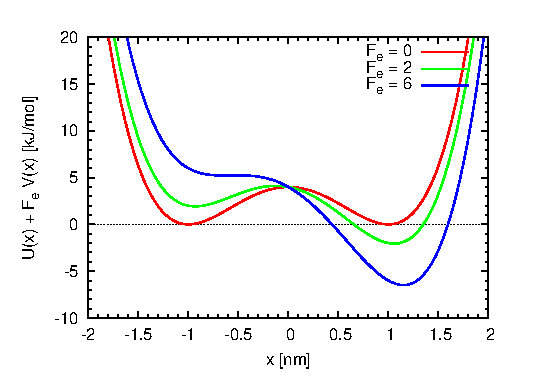
\includegraphics[width=8cm]{./fig.md/fig-pot.eps}
  \caption{The original dihedral potential and the dihedral potential
    with optimal control potential.}
  \label{fig:tmp2}
\end{figure}


We considered $T = 1.0$, 0.5, 0.2 and 0.1~ps. The results of the importance sampling computations are shown in Fig.~\ref{fig:tmp2}, Tab.~\ref{tab:tmp1} and Tab.~\ref{tab:tmp2}.
From each of the 5,000 equilibrium system states from the \emph{gauche} conformation, 4 trajectories with
different random seeds are simulated for each $T$, so we
generate $M_{IS}=20,000$ trajectories for $T = 1.0$, 0.5, 0.2.
For $T = 0.1$~ps, 12 trajectories are simulated from each
initial system state, so 60,000 trajectories in total.
The optimal control $u(r, \omega)$ is
calculated by simulations of butane in vacuum, in which all other
parameters are the same as the aforementioned descriptions, except
that the water molecules are removed. This is done because the vacuum
simulation is much cheaper than the in-water simulation, and
practically, the control calculated in the corresponding vacuum
systems performs well enough in the in-water system, because we find, when tested,
 no further iteration is needed to refine the control. In the vacuum system, we find  probabilities $\bP(\tau\leq T) =
2.16\times10^{-2}$, $8.66\times 10^{-3}$, $1.48\times 10^{-3}$ and
$6.13\times 10^{-5}$ for $T = 1.0$, 0.5, 0.2 and 0.1~ps,
respectively. These values do not significantly differ from those of the
dissolved system (see the second column of Tab.~\ref{tab:tmp1}).
Noticing that butane is invariant with respect to transitional and
rotational movement, the above observations  indicate that
the transitional, rotational DOFs and the water structure do not
play a dominant role in the conformational change of butane, and the
definition of control only as a function as the dihedral angle, and
the computation of control in the vacuum system are reasonable
choices.  

\begin{table}[t]
  \centering
  \caption{
    Results for butane dissolved in water: The probability
    $\bP (\tau \leq T)$ is calculated by the importance sampling procedure with
    control acting on the dihedral angle only; see the text for more details.
    The column ``Error'' denotes the statistical uncertainty of
    estimating the probablity $\bP (\tau \leq T)$.
    If the  trajectories are statistically independent, the expected error is $\sqrt{\textrm{Var}/M_{IS}}$, where
    $M_{IS}$ is the number of trajectories used. If the trajectories are not independent, the error
    can be estimated by the block average method~\cite{frenkel2001understanding}.
    The meaning of the other columns are the same as Tab.~\ref{tab-ex1-2}. 
    %here, the accelaration index has to be computed as  $\cI=\textrm{Var}_{MC} M_{MC}/(\textrm{Var}_{IS}M_{IS})$ since the numbers of trajectories used in the IS and MC procedures are different.
  }
  \label{tab:tmp1}
  \begin{tabular*}{0.9\textwidth}{@{\extracolsep{\fill}}lcccrr}
    \hline\hline
    $T$ [ps] & $\bP (\tau \leq T)$ & Error & Var & Accel. $\cI$ & Traj. Usage \\\hline
    0.1 & $4.30\times 10^{-5}$ & $0.77\times 10^{-5}$ & $3.53\times10^{-6}$ & 12.2 & 0.4\%\\
    0.2 & $1.21\times 10^{-3}$ & $0.11\times 10^{-3}$ & $2.50\times10^{-4}$ & 4.8 & 5.4\%\\
    0.5 & $6.85\times 10^{-3}$ & $0.38\times 10^{-3}$ & $2.88\times10^{-3}$ & 2.4 & 8.3\%\\
    1.0 & $1.74\times 10^{-2}$ & $0.08\times 10^{-2}$ & $1.21\times10^{-2}$ & 1.4 &12.3\%\\
    \hline\hline
  \end{tabular*}

%%HERE
  \caption{
    Results for butane dissolved in water: Brute force / standard Monte Carlo computations of $\bP (\tau \leq T)$ 
    without any importance sampling.}\label{tab:tmp2}
  \begin{tabular*}{0.9\textwidth}{@{\extracolsep{\fill}}lcccrr}
    \hline\hline
    $T$ [ps] & $\bP (\tau \leq T)$ & Error & Var & Accel. & Traj. Usage \\\hline
    0.1 & $9.00\times 10^{-5}$ & $3.00\times 10^{-5}$ & $9.00\times10^{-5}$ & 1.0 & 0.009\%\\
    0.2 & $1.29\times 10^{-3}$ & $0.11\times 10^{-3}$ & $1.29\times10^{-3}$ & 1.0 & 0.1\%\\
    0.5 & $7.41\times 10^{-3}$ & $0.27\times 10^{-3}$ & $7.36\times10^{-3}$ & 1.0 & 0.7\%\\
    1.0 & $1.78\times 10^{-2}$ & $0.04\times 10^{-2}$ & $1.75\times10^{-2}$ & 1.0 & 1.8\%\\
    % 0.2 & $7.46\times 10^{-4}$ & $2.36\times 10^{-4}$ & $7.46\times10^{-4}$ & 1.0 & 0.1\%\\
    % 0.5 & $6.94\times 10^{-3}$ & $0.72\times 10^{-3}$ & $6.89\times10^{-3}$ & 1.0 & 0.7\%\\
    % 1.0 & $1.61\times 10^{-2}$ & $0.11\times 10^{-2}$ & $1.59\times10^{-2}$ & 1.0 & 1.6\%\\
    \hline\hline
  \end{tabular*}
\end{table}

In Fig.~\ref{fig:tmp1} the effective dihedral angle energy is plotted being defined as the original dihedral energy $V_\phi(\phi)$ plus the control
$V_{\textrm{ctrl}}(\phi)$. We only show the effective energy in the
range $[40^\circ, 150^\circ]$, because the initial states of the trajectories are located in the range $[40^\circ, 80^\circ]$, and the
trajectories are stopped when they reach $\phi = 150^\circ$. For an easy
comparison, all effective energies are shifted by a constant, so that
they are of  value zero at $\phi = 150^\circ$. It clear that for
smaller $T$ values, the control applied is stronger.  The
resulting probabilities $\bP (\tau \leq T)$ calculated by the
importance sampling procedure are summarized in Tab.~\ref{tab:tmp1},
which is consistent with Tab.~\ref{tab:tmp2} that presents the
brute force results (calculated from $M_{MC}=100,000$ trajectoies).
The consistency at $T = 0.1$~ps is worse, because
among the 100,000 trajectoies, only 9 of them hit the \emph{trans}
conformation within 0.1~ps, therefore both the estimate of the probability
$\bP (\tau \leq T)$ and its error are not reliable due to the
insufficient sampling.
Since the variance is reduced, the error of the
statistical estimate is more precise in the importance sampling case. The
reduced variance is shown in the fourth column of Tab.~\ref{tab:tmp1},
which is much smaller than the brute force case (the fourth column of
Tab.~\ref{tab:tmp2}). The fifth column presents the acceleration index $\cI$
of the importance sampling procedure relative to standard Monte Carlo. It measures the speed-up gained by the
importance sampling. The column "trajectory usage"
presents the percentage of the trajectories that changes to the \emph{trans}
conformation within time interval $[0, T]$. It is increased by
the control with respect to the brute force result.




\section{Discussions}
\label{sec-discuss}

As a continuation of our works \cite{zlph2013, zhws13}, we propose a cross-entropy
algorithm for diffusion processes and study its application to
importance sampling and optimal control.
For instance, in our previous work  \cite{zhws13}, we have analysed the effect of the use of suboptimal controls in multiscale systems with explicit scale separation, e.g., slow-fast systems or diffusions in the small-noise limit. Here the situation is different, in that no such small parameter or detailed information regarding the relevant degrees of freedom is used.  On the other hand, in the cross-entropy method, the approximation of the target measure and, consequently, effcient importance sampling or control strategies crucially depend on a sensible choice of a function basis. 
%
A good choice can be often based on prior knowledge about the dynamical
system, such as metastable states or reactive cordinates; it is easy to
imagine that there is no way to obtain satisfactory results when the basis functions used are not supported along the relevant degrees of freedom.
The relation between the cross-entropy method and methods for multiscale dynamical systems is an interesting and yet open question that will be addressed in future work.

\section*{Acknowledgement}
The authors acknowledge financial support by the DFG Research Center MATHEON.
\FloatBarrier

\bibliographystyle{siam}
\bibliography{reference}
\end{document}